\documentclass{article}

\usepackage[utf8]{inputenc}
\usepackage[T1]{fontenc}
\usepackage{graphicx}
\usepackage{amsmath}
\usepackage[margin=1in]{geometry}
\usepackage{titlesec}
\usepackage{enumitem}

\titleformat{\section}
{\LARGE\bfseries}{\thesection}{1em}{}

\titleformat{\subsection}
{\Large\bfseries}{\thesection}{1em}{}

\begin{document}

\pagestyle{empty}

\section*{Il modello relazionale}
\large
Esiste una archittetura standard conseguita nei DBMS articolata su \textbf{tre livelli}, detti rispettivamente \textbf{logico}, \textbf{interno} ed \textbf{esterno}, di cui di seguito si analizzano le caratteristiche:
\begin{enumerate}
    \renewcommand{\labelenumi}{-}
    \itemsep0em
    \item \textbf{Schema Esterno}: costituisce la descrizione di una porzione di interesse del \textit{data base} usufruendo del \textit{modello logico}
    \item \textbf{Schema Logico}: costituisce una descrizione dell'intera basi di dati per mezzo del \textit{modello logico} adottato dal DBMS
    \item \textbf{Schema Interno}: costituisce la rappresentazione dello \textit{schema logico} per mezzo di strumenti di memorizzazione, indicando come gli stessi dati debbano essere veramente organizzati, gestiti poi consecutivamente dal DBMS \textit{(spesso le strutture dati usate sono strutture fisse, strutture variabili oppure grafi)}
\end{enumerate}
\begin{center} 
    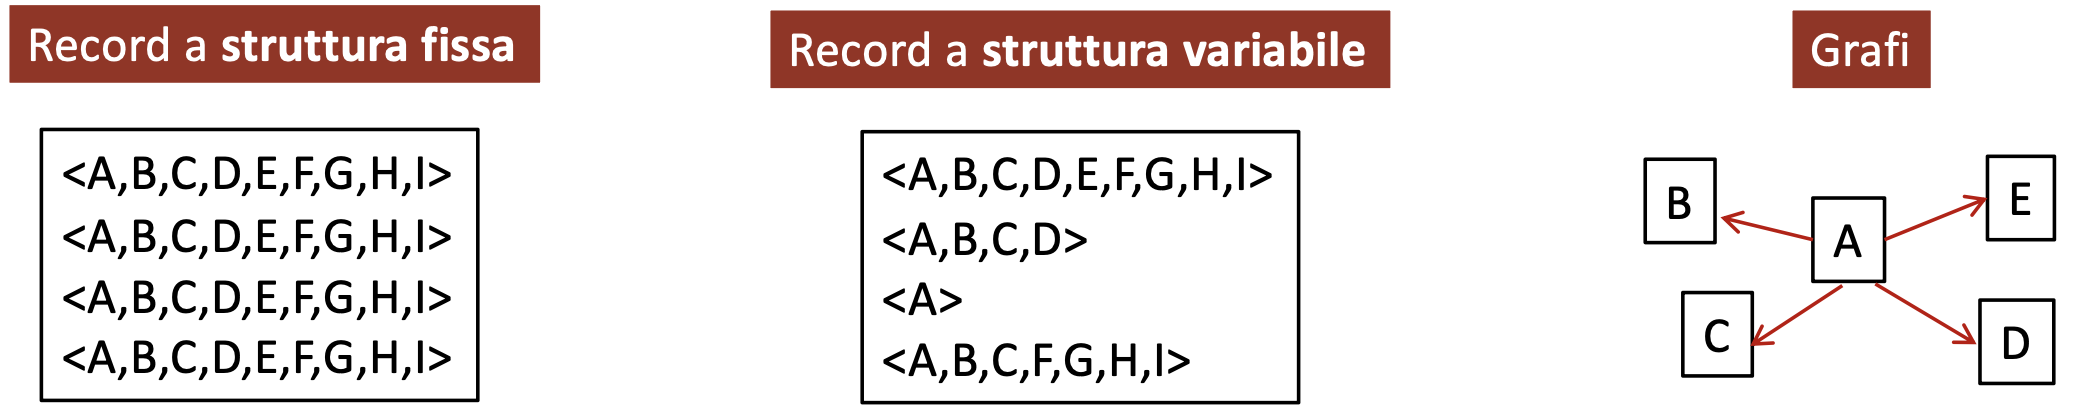
\includegraphics[width=0.7\textwidth]{foto 1.png}
\end{center}

\subsection*{Modello Logico}
\large 
Il \textit{modello logico} pone un formalismo qualora i dati siano accettabili o meno, ossia se possano essere memorizzati all'interno delle relazioni o tabelle. Tuttavia è bene considerare come tale \textit{formalismo} indica regole generali a cui attenersi, indipendentemente dal \textit{data base} creato.\vspace{14pt}\\Un semplice esempio è favorito dalla creazione di relazioni in grado di mantenere al loro interno dati riferiti a voti di esame; un vincolo potrebbe essere dato dal fatto che possano essere memorizzati valori che abbiano una votazione maggiore o uguale 18 e inferiore o uguale a 30L per essere memorizzati nel \textit{data base}.
\vspace{14pt}\\Ogni singola progettazione di un DBMS è relativa all'impegno di due \textbf{proprietà}, le quali possono essere adottate come dei veri e propri \textit{vincoli}, quali:
\begin{enumerate}
    \renewcommand{\labelenumi}{-}
    \itemsep0em
    \item \textit{Indipendenza fisica}: ossia un programma non deve conoscere l'\textit{organizzazione fisica} dei dati
    \item \textit{Indipendenza logica}: un programma può vedere i dati tramite opportuni \textit{schemi esterni}, quali relazioni o view
\end{enumerate}
Differenti sono i \textit{modelli logici} adottati, ma dove principalmente sono adoperate due grandi famiglie quali: \textbf{modelli relazionali} e \textbf{modelli scheme-less}, dei due il primo citato risulta il più diffuso.

\subsection*{Modello Relazionale}
\large
Le ragioni principali che rendono il \textbf{modello relazionale} il più utilizzato sono:
\begin{enumerate}
    \renewcommand{\labelenumi}{-}
    \itemsep0em
    \item garantisce la separazione tra il livello fisico e logico
    \item è caratterizato da un uso intuitivo, connesso a forti fondamenta legate ad algebra di base
\end{enumerate}\vspace{14pt}
\textit{Definizione informale}\\I dati sono organizzati in \textit{record} di dimensione fissa, e divise in \textit{tabelle}, dette \textbf{relazioni}.\vspace{14pt}\\Come citato dalla definizione, le strutture usate per salvare qualunque dato sono definite \textit{record}, memorizzati all'interno di una tabella. La dimensione è \textit{fissa}, poichè per ogni singolo record è mantenuto lo stesso numero di \textbf{attributi}, ossia la stessa molteplicità di \textit{colonne}. Inoltre il connubio dettato dal [\textit{nome tabella} e \textit{nome attributi}] indica lo \textbf{schema} della relazione; infine, i record o le \textit{righe} della tabelle sono denominate \textbf{istanze} della relazione.
\begin{center}
    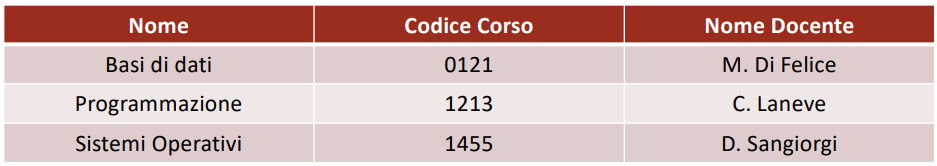
\includegraphics[width = 0.7\textwidth]{foto 2.png}
\end{center}
Il modello relazionale gode di alcuni \textit{vincoli}, i quali non possono essere raggirati pur di ottenere una struttura corretta del data base. Tali vincoli sono:
\begin{enumerate}
    \renewcommand{\labelenumi}{-}
    \itemsep0em
    \item L'\textbf{ordinamento} delle righe, come anche delle colonne, è irrilevante, l'importanza ricade solo sul contenuto
    \item Non possono esistere \textbf{attributi uguali}
    \item Non possono esistere \textbf{righe uguali}
    \item I dati di ogni colonna devono essere \textbf{omogenei} fra loro
\end{enumerate}
Ponendo uno sguardo sulle colonne, ogni attributo dispone di un \textbf{dominio}, che definisce l'\textit{insieme di valori validi} per quell'attributo, inoltre, differenti attributi possono condividere lo stesso dominio. Un esempio può essere (dom(Nome) = string).\vspace{14pt}\\
I dati gestiti dal modello relazionale oltre ad essere omogenei fra loro, qualora posti nella stessa colonna, sono \textbf{dati strutturati}, tutti i valori della stessa tabella condividono la stessa struttura, quindi non sarà mai possibile gestire istanze che abbiano un numero inferiore di domini.\vspace{14pt}\\
Sono stati osservati i vincoli principali su cui pone la realizzazione e concretizzazione dello scheletro della base di dati, tuttavia spesso l'importanza ricade sul rispetto della \textbf{Prima Forma Normale}.\\La \textit{Prima Forma Normale} indica delle proprietà che una qualsiasi relazione deve disporre. Innanzitutto è stabilito come ogni attributo sia definito su un \textit{dominio atomico} e non su \textit{domini complessi}; ossia, i dati memorizzati non possono essere valori combinati fra loro, da cui solitamente sono adoperati processi di \textit{normalizzazione} per rendere ogni attributo atomico.\\
Ulteriore regola, ma non vincolante, indica la buona pratica di evitare la ripetizione di stessi dati per poter occupare il minimo spazio di memoria; infatti, la strategia adottata da modelli relazionali è garantita dall'uso di puntatori, dove la visualizzazione di stessi dati in differenti tabelle, non è da imputare alla maggiore memoria occupata, ma rispetto a stessi riferimenti a celle di memoria.\\ 
Spesso capita di osservare medesime informazioni contenute in differenti relazioni le quali sono \textbf{correlate} logicamente fra loro, dove nel modello relazionale questi riferimenti sono costruiti mediante gli stessi \textbf{valori}.
\begin{center}
    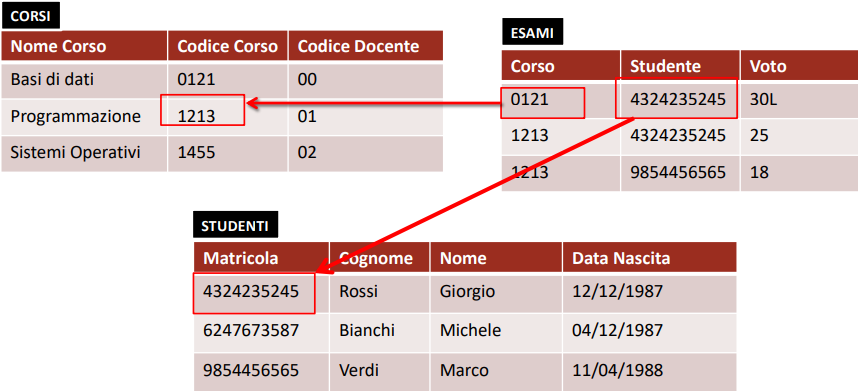
\includegraphics[width = 0.7\textwidth]{foto 3.png}
\end{center}
Tuttavia nella \textbf{pratica} la progettazione di una base di dati non traduce a priori le informazioni di interesse in un modello relazionale.\ Tipicamente ciò che è noto sono i requisiti funzionali e non il modello relazionale; occorre quindi individuare una serie di passaggi che rendano concreto lo sviluppo del modello logico.\\
La nozione di relazione come sinonimo di tabella in questo contesto non è da tralasciare. In ambito matematico una relazione può essere definita come un sottoinsieme del prodotto cartesiano di una qualsiasi coppia di insiemi.\ Tuttavia occorre descrivere il concetto di relazione in maniera più formale.
\subsection*{Relazione matematica}
\large
\textit{Definizione}\\Il \textbf{prodotto cartesiano} degli insiemi \textit{$D_1$}, \textit{$D_2$}, \textit{...}, \textit{$D_N$} è definito come l'\textbf{insieme delle tuple ordinate} (\textit{$d_1$}, \textit{$d_2$}, \textit{...}, \textit{$d_N$}), con \textit{$d_i$} $\in$ \textit{$D_i$}, $\forall$ \textit{i} $\in$ \textit{1, 2, ..., n}.\vspace{14pt}\\
Per esempio, dati gli insime \textit{A = [1, 2, 4]} e \textit{B = [a, b]}, il prodotto cartesiano dei due insiemi è costituito dall'insieme di tutte le possibili coppie in cui il primo elemento appartiene ad \textit{A} e il secondo a \textit{B}. Si ottengono così sei coppie:\
\vspace{-\baselineskip}
\begin{center}
    \item (1, a), (1, b), (2, a), (2, b), (4, a), (4, b)
\end{center}
\vspace{14pt}
\textit{Definizione}\\Dati \textit{n} insiemi \textit{$D_1$}, \textit{$D_2$}, \textit{..., $D_N$} una \textbf{relazione matematica} sugli insiemi \textit{$D_1$}, \textit{$D_2$}, \textit{...}, \textit{$D_N$} è definita come un \textbf{sottoinsieme del prodotto cartesiano} \textit{$D_1$} x \textit{$D_2$} x \textit{...} x \textit{$D_N$}.\vspace{14pt}\\
Quindi una\ \textit{relazione matematica} sugli insiemi \textit{A} e \textit{B} è un sottoinsieme di \textit{A $\cdot$ B}, questo sottoinsieme, a livello semplificativo, può essere:
\vspace{-\baselineskip}
\begin{center}
    \item (1, a), (1, b), (2, a), (2, b), (4, a), (4, b)
\end{center}
\vspace{14pt}
Il numero di elementi della relazione viene chiamato \textit{cardinalità} della relazione. Mediante la stessa cardinalità sono adottate ulteriori annotazioni affini rispetto all'ambito di relazioni e tabelle. Rispetto alla teoria degli insiemi, sono stabilite alcune operazioni tipiche, le stesse sfruttate anche in questo contesto:
\begin{enumerate}
    \renewcommand{\labelenumi}{-}
    \item \textit{Intersezione}: il sottoinsieme conterrà al suo interno solo elementi che risultino essere in comune tra qualsiasi totalità di insiemi dati. Dove di seguito è riportata la cardinalità dell'insieme:
    \vspace{-\baselineskip}
    \begin{center}
        \item |A $\cap$ B| = \{0, min(|A|, |B|)\}
    \end{center}
    \item \textit{Unione}: il sottoinsieme conterrà tutti gli elementi, eccetto i duplicati, rispetto agli insiemi presi in considerazione. Dove di seguito è riportata la cardinalità:
    \vspace{-\baselineskip}
    \begin{center}
        \item |A $\cup$ B| = \{max(|A|, |B|), |A| + |B|\}
    \end{center}
    \item \textit{Differenza}: il sottoinsieme conterrà gli elementi del primo insieme preso in considerazione eccetto quelli corrisposti all'interno del secondo insieme.\ Dove di seguito è riportata la cardinalità:
    \vspace{-\baselineskip}
    \begin{center}
        \item |A $\backslash$ B| = \{0, |A|\}
    \end{center}
    \item \textit{Prodotto Cartesiano}: il sottoinsieme conterrà gli elementi del primo insieme e del secondo insieme. Dove di seguito è riportata la cardinalità:
    \vspace{-\baselineskip}
    \begin{center}
        \item |A $\cdot$ B| = \{|A| $\cdot$ |B|\}
    \end{center}
\end{enumerate}
Quindi una tabella può essere osservata come un sottoinsieme del prodotto cartesiano, anche se risulta contradditorio dal punto di vista simmetrico. Infatti, a livello di definizione, indicare il prodotto cartesiano A $\cdot$ B oppure B $\cdot$ A \textbf{non stabilisce} la stessa entità, anche se ciò, tradotto rispetto ad una rappresentazione grafica, si rispecchia in un posizionamento differente delle colonne o domini all'interno delle relezioni.

\subsection*{Informazioni incomplete}
\large
All'interno di una relazione, le \textbf{ennuple} di dati, ossia le differenti \textit{row}, devono essere omogenee fra loro.\ Tuttavia, in alcuni casi, l'\textit{attributo} associativo per una determinata \textit{ennupla} potrebbe non essere noto o addirittura inesistente.\vspace{14pt}\\
Una soluzione consiste nel battezzare \textit{valori speciali}, ossia colmare informazioni mancanti. Un primo approccio è dato dalla creazione di valori speciali per ogni attributo oppure, molto più utilizzato, etichettare tutto ciò che sia mancante con il \textbf{valore NULL}.
Il valore \textit{NULL} garantisce una netta soluzione per dati mancanti, tuttavia è buona pratica limitarne il numero, a causa dell'elevato spreco di memoria che potrebbe provocare. Nella progettazione di basi di dati esiste un \textit{trade-off} tra le tabelle e il valore NULL, ossia comporre ulteriori relazioni, differenziando in questo modo record che siano in grado o meno di compensare tutti i domini richiesti.

\subsection*{Vincoli di integrità}
\large
Una fase fondamentale è data dalla capacità di stabilire quali istanze possano essere \textbf{inserite} all'interno di una tabella.\ Infatti, molto spesso, alcuni record di una relazione possono considerarsi illeciti, ossia sono caratterizzati da valori posti al di fuori delle restrizioni fissate dai differenti attributi dello \textit{schema} della base di dati.\vspace{14pt}\\
Perciò è adottato un meccanismo in grado di provvedere alla problematica precedente, mediante la nozione di \textbf{vincolo}.\vspace{14pt}\\ 
\textit{Definizione informale}\\Un \textit{vincolo} è una funzione booleana, che associa ad una istanza di una base di dati un \textbf{valore di verità}.\vspace{14pt}\\
Per cui un vincolo predispone quali siano istanze lecite o meno, ossia se soddisfino tutti i requisiti; solamente soddisfatti tutti i vincoli sarà possibile inserire l'istanza nella relazione. Tendenzialmente si adotta una duplice suddivisione tra \textit{vincoli intra-relazionali}, ossia relativi alla stessa relazione, e \textit{vincoli inter-relazionali}, tra relazioni differenti.

\subsection*{Vincoli intra-relazionali}
\large
Come già detto i \textbf{vincoli intra-relazionali} considerano una singola tabella. A loro volta si suddividono in due entità:
\begin{enumerate}
    \renewcommand{\labelenumi}{-}
    \item \textit{Vincoli di ennupla}: regole poste su ciascuna riga della tabella, quali espressioni algebriche oppure funzioni booleane.\ Se l'espressione o funzione adoperata dovesse corrispondere un risultato negativo relativo alla caratterizzazione del nuovo record da memorizzare, non sarà consentito l'inserimento dell'istanza all'interno della relazione.
    \item \textit{Vincoli di chiave}: requisiti posti sulle colonne o domini, i quali a loro volta si intrecciano rispetto a tre possibili definizioni, per cui sono vincoli più articolati rispetto ai precedenti.
\end{enumerate}
Un \textbf{vincolo di chiave} si articola in tre definizioni consecutive. La prima osservata è in relazione al concetto di \textbf{superchiave}.\vspace{14pt}\\
\textit{Definizione informale}\\ Una \textit{superchiave} è una colonna o più colonne se non sono presenti valori ripetuti o duplicati.\vspace{14pt}\\
Il concetto di \textbf{chiave} è adoperato per rendere univoca, durante una qualsiasi fase di ricerca, una ennupla, prendendo in considerazione un insieme di possibili attributi. Per cui, come da definizione, la \textit{superchiave} è in grado di rispettare quanto voluto, tuttavia la decisione di quali colonne scegliere deve garantire la mancanza di istanze identiche, altrimenti provocherebbe un dissenso rispetto all'univocità.\\
E' buona pratica progettare le chiavi a livello di schema, ossia osservando la struttura della relazione cercando di accomunare tutte le istanze. Tuttavia la creazione di una \textit{superchiave} potrebbe prendere in considerazione colonne ridondanti, ossia rendere istanze univoche ma utilizzando attributi non affini all'obiettivo di una \textit{chiave}. Per questo si adopera il passaggio da \textit{superchiave} a \textit{superchiave minimale}.\vspace{14pt}\\
\textit{Definizione informale}\\ Una \textit{chiave} è una superchiave minimale di \textit{r}, ossia della relazione. \vspace{14pt}\\
Per fare in modo di ottenere una \textit{chiave minimale}, occorre che la scelta su cui ricade il numero di colonne sia il minimo possibile; per cui presi in considerazione certi attributi, la progettazione della chiave avviene osservando se preso un numero sempre più ristretto di attributi sia possibile o meno rendere una qualsiasi ennupla univoca durante una qualsiasi operazione. Scegliere una \textit{chiave} piuttosto di una superchiave avviene per rendere maggiormente facile la correlazione ad ennuple e la connesione tra differenti relazioni.\ Un esempio associato a tale contesto potrebbe essere dato dalla presenza piuttosto consistente di valori NULL nella tabella. I valori NULL, come già detto, potrebbero rappresentare un'arma a doppio taglio; infatti ipotizzando quanto detto, non è più vero che le chiavi riescano a identificare unicamente le differenti istanze e a stabilire connesioni tra relazioni.\\
E' necessario introdurre un ulteriore meccanismo che vieti l'uso di valori NULL per la costruzione di superchiavi minimali.\vspace{14pt}\\
\textit{Definizione informale}\\Una \textit{chiave primaria} è una chiave, ossia rappresenta già una superchiave e una superchiave minimale, di una relazione su cui non sono ammessi valori NULL.\vspace{14pt}\\
Quindi l'uso di \textit{chiavi primarie} risulta essere la soluzione migliore, permette univocità delle ennuple e le connessioni tra relazioni.\ Tuttavia, a volte potrebbe capitare che sia impossibile scegliere attributi che non abbiano valori NULL.\ Semplicemente, si adottano degli \textit{identificativi progressivi}, ossia attributi di tipo intero, i quali in completa autonomia ad ogni nuovo inserimento di istanze corrette associa un valore incrementato, rendendo così unico il collegamento.
\begin{center}
    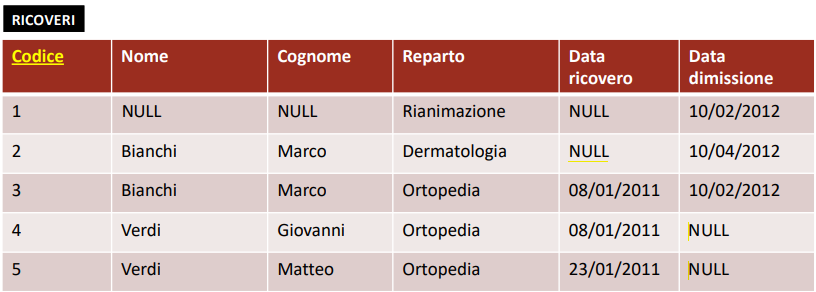
\includegraphics[width = 0.6\textwidth]{foto 4.png}
\end{center}

\subsection*{Vincoli inter-relazionali}
\large
Un modello relazionale è adottato soprattutto per garantire molte connessioni fra relazioni della stessa base di dati, collegamenti espressi mediante attributi di differenti tabelle dello stesso tipo.\ Per cui, potrebbe risultare utile porre delle \textbf{restrizioni} sulle \textit{dipendenze} tra relazioni.\vspace{14pt}\\
\textit{Definizione informale}\\Ogni \textbf{riga} della tabella \textbf{referenziante} si collega al \textbf{massimo} ad un \textbf{riga} della tabella \textbf{referenziata}, sulla base di simili attributi scelti per porre un punto in comune.\vspace{14pt}\\
Il \textbf{vincolo di integrità inter-relazionale} interviene proprio per determinare delle regole a cui sottostare.\vspace{14pt}\\
\textit{Definizione informale}\\Un \textit{vincolo di integrità referenziale} fra gli attributi X di una relazione $R_1$ e una relazione $R_2$ impone ai valori, diversi da NULL per definizione, X di $R_1$ di comparire come valori della \textit{chiave primaria} di $R_2$.
\begin{center}
    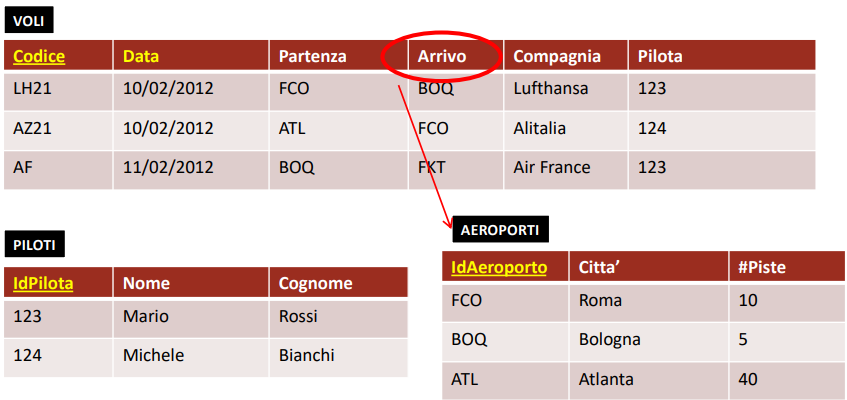
\includegraphics[width = 0.7\textwidth]{foto 5.png}
\end{center}
Come da immagine, in pratica, il vincolo consente di collegare fra loro relazioni mediante stessi dati che siano dello stesso dominio; considerando che tali valori nella tabella referenziante siano posti non necessariamente nella chiave primaria, contrariamente rispetto alla relazione referenziata, la quale deve mantenere i dati fittizzi all'interno del dominio che componga la propria chiave primaria.\vspace{14pt}\\
Potrebbe accadere che durante una fase di \textit{aggiornamento}, alcuni record che compongono referenze fra relazioni vengano eliminati, oppure poste delle modifiche che violino i vincoli di integrità. In considerazione a quanto detto si adottano tre strategie:
\begin{enumerate}
    \renewcommand{\labelenumi}{-}
    \item \textbf{NON} consentire l'operazione, qualora riguardi istanze utilizzate per la costruzione di referenze tra relazioni
    \item \textbf{Eliminazione a cascata}, ossia l'eliminazione di record all'interno della relazione \textit{referenziante} deve provocare l'eliminazione delle stesse istanze utilizzate nella relazione \textit{referenziata}, e viceversa
    \item \textbf{Inserimento} dei valori \textbf{NULL}, questo accade nei confronti di entrambe le relazioni che compongano la referenza, quindi eliminati determinati record occorre inserire nella tabella di riferimento nei corretti domini il valore di carattere speciale
    \begin{center}
        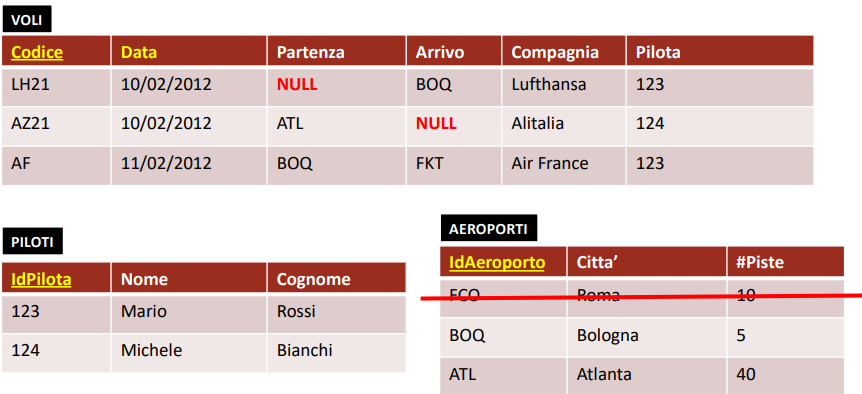
\includegraphics[width = 0.6\textwidth]{foto 6.png}
    \end{center}
\end{enumerate}
\end{document}